\section{Neural network theory}
The artificial neuron is a mathematical model that was originally proposed in 1943 in \citeauthor{McCulloch1943} \autocite{McCulloch1943}.
Starting in the 1980s, efficient and effective variations of the basic model were published, and around the 1990s these types of techniques became more popular due to the high computing power provided by new computers.

Originally, the proposal was a simplification of the biological neuron model, known as the artificial neuron. It is based on one or more binary inputs and a single binary output. The artificial neuron "activates the output" when a certain number of inputs are active. The connection, or edge, between two neurons or between an input and a neuron is called a link. Each link is associated with a Boolean value that can be either 0 or 1. With this infrastructure, neurons can perform operations based on the traditdional logic operators AND, OR or NOT.
Figure ~\ref{fig:neuronsBasic} depicts the architecture consisting of a single neuron with a single output and one or more inputs.

\begin{figure} [h]
    \centering
    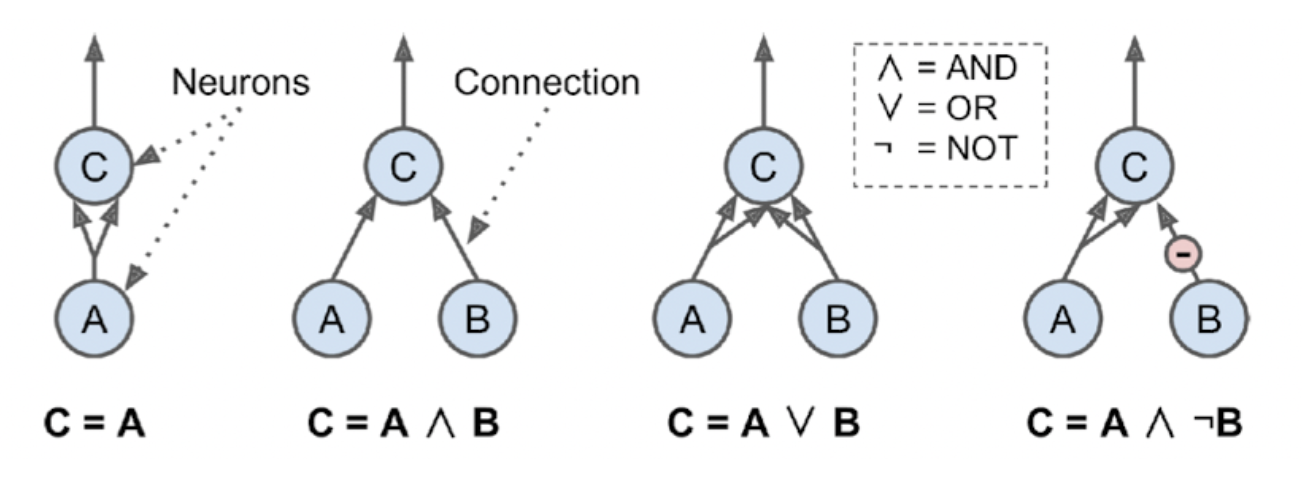
\includegraphics [width=\textwidth,height=\textheight,keepaspectratio] {Images/Theory_and_method/unnamed.png}
    \caption{ Scheme of a classical artificial neuron capable of implementing boolean algebra.}
    \label{fig:neuronsBasic}
\end{figure}

\clearpage

\section{The perceptron and multilayer perceptron} \label{percy}
The perceptron is one of the simplest ANN (artificial neural network) architectures. It was invented in 1957 by Frank Rosenblatt. It is based on a neuron called threshold logic unit (TLU) connected to inputs and with only one output link. The inputs and outputs, instead of binary values as in the classical model, are scalar numbers and each link is associated with a weight. The TLU computes a weighted linear combination of the inputs called z $\left(z=w_{1} x_{1}+w_{2} x_{2}+\ldots+w_{n} x_{n}= {\bf x^{t} w}\right)$.

After this input, the step function is applied to the summation represented by z. Formally, this procedure takes place as shown in Eq \eqref{formula} and Figure ~\ref{fig:summatory}.

\begin{equation} 
    h_{w}({\bf x}) = step(z), where \:z = {\bf x^{t} w}
    \label{formula}
\end{equation} 

\begin{figure} [h]
    \centering
   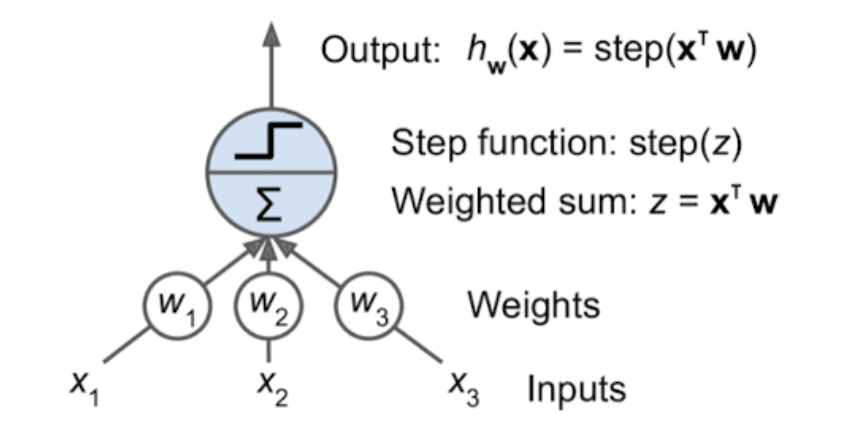
\includegraphics[width=\textwidth,height=\textheight,keepaspectratio]{Images/Theory_and_method/unnamed-2.png}
    \caption{Scheme of a Perceptron cell.}
    \label{fig:summatory}
\end{figure}

The most common step function is the heaviside (or step function). In this case,it is used to determine the activation of the neuron based on the output of the linear combination, as shown in Eq \eqref{Heaviside function}: 
\begin{equation} 
    \text { heaviside }(z)=\left\{\begin{array}{l}
    0 \text { if } z<0 \\
    1 \text { if } z \geq 0
    \end{array}\right.
    \label{Heaviside function}
\end{equation} 

In this equation:
\begin{itemize}
    \item \textbf{X} represents the input feature matrix.
    \item \textbf{W} represents the matrix of weights. It contains all the weights except the bias neuron.

    \item \textbf{b} is a vector that contains all the weights between the bias neuron and the artificial neuron (it contains the distortions between the results and reality).
    \item \textbf{$\phi$} is called an activation function. Which is the step function in the case of the Multilayer Perceptron.
\end{itemize}

Regarding the learning phase, a learning rule that was largely inspired by Hebb's rule, introduced in \citeauthor{Morris1999} \autocite{Morris1999}, is used. In the text it is said that, in nature, when a biological neuron is activated, it consequently activates or triggers another neuron, the connection between the two becomes greater. The perceptron is trained with a variant of this concept that takes into account the errors made by the network when making predictions. The learning rule reinforces connections that help reduce error and reduces those that contribute to increased error. Eq \eqref{bohfoormula} represents the the learning rule.

\begin{equation}
w_{i,j}^{\text{(next step)}} = w_{i,j} + \eta(y_j - \hat{y}_j) x_i
\label{bohformula}
\end{equation}

\begin{itemize}
    \item $w _{i, j}$ is the connection weight between to given neurons.
    \item $x_{i} $ is the value of the input.
    \item $ŷ _{j}$ is the interpolated value of the output.
    \item $y_{j}$ is the observed value of the output.
    \item $\eta$ is the learning rate.
\end{itemize}

\clearpage

\section{Backpropagation and parameter optimization} \label{backprop}
Error backpropagation is an algorithm used for training artificial neural networks, which is used as a method for stochastic gradient descent and thus enables error reduction in the learning process. The term backpropagation refers only to the algorithm for computing the gradient, not to describe how the gradient is used.

The learning phase therefore consists in finding the optimal parameters that create the best model, and an iterative approach is used to do this by gradually modifying the parameter values with respect to the previous iteration.

This training mechanism starts with random initialization of the parameters and is carried out using input-output pairs until a minimum of the cost function, which is responsible for calculating the error, is reached. Each iteration is called an epoch.
The optimization procedure is as follows:
\begin{itemize}
    \item The weights and biases of the network are initialized with random values.
    \item These parameters are iteratively optimized. This phase consists in 4 subphases:
    \begin{itemize}
        \item The model prediction is calculated using the current parameters.
        \item The cost function, that drives the optimization process, is applied to the obtained output with respect to the expected output.
        \item The gradient, which will be used to determine how to tweak the parameters, is calculated with respect to the cost function through the process of backpropagation.
        \item The parameters are updated. 
    \end{itemize}
\end{itemize}

These four steps can be repeated for an arbitrary number of iterations, and the process is usually stopped when a local minimum is reached.
\clearpage 
\section{Hyperparameters} \label{hyperdescrp}
While the values of a neural network’s parameters, namely its weights and biases, are defined by its training process, there’s a set of different parameters, called hyperparameters, that are not optimized by the learning process. 
The hyperparameters of a neural network define its architecture and the characteristics of its learning phase. They act as factors, external to the learning phase, that have an impact on the model’s performance.
The most important hyperparameters are the following:
\begin{itemize}
    \item \textbf{Batch}
    \\When Stochastic Gradient Descent (SGD) is used, the parameters are updated after each sample of the dataset is evaluated in the training phase. This approach is considered significantly noisy since the gradient descent direction derived by one sample might differ from the direction derived from other samples, significantly increasing the variance across the different iterations of the learning process.
    \\Generally speaking, the model gets updated after a specific number of samples has been processed. This is known as the batch size of samples.  SGD can therefore be seen as having a batch size of one.
    In addition to being less noisy, the use of batch sizes greater than one results in reduced training times if paired with the use of GPUs or other specialized hardware. Moreover, the optimization towards a minimum will likely be less erratic than in the case of SGD, increasing the chances of actually converging.

    \item \textbf{Epoch}
    \\An epoch in machine learning means one complete pass of the training set through the algorithm, that is, its propagation through the network’s architecture. Normally an epoch is divided into one or more batches. The number of epochs and batches per epoch are both integers.
    \\There’s no limit to the amount of epochs to use in the training process, which can thus take up an arbitrary amount of time. To stop the algorithm from running, a fixed number of epochs can be used. Alternatively, early-stopping can be used, which consists of stopping the training as soon as the validation error stops showing significant improvements after a predetermined number of epochs, referred to as patience. As a consequence, the number of epochs can be set to a big integer to give ample room for the training to take place, while relying on early-stopping to stop when appropriate.
    \item \textbf{Number of hidden layers}
    \\As explained in chapter ~\ref{percy}, the number of hidden layers is determined by the amount of layers between the input and output layers.
    \item \textbf{Number of neurons per layer}
    \\The number of neurons in input and output layers is determined by the type of the input and output necessary for the task at hand. For the hidden layers, on the other hand, it used to be common to structure them into a pyramid-shaped, with fewer and fewer neurons at each layer. For instance, a neural network could have 3 hidden layers, the first one with 300 neurons, the second with 200 neurons and the last with 100. 
    This practice, however, is not used anymore because it’s been empirically proven that using the same number of neurons in all hidden layers performs just as well in most cases.
    \item \textbf{Learning rate}
    \\It determines the step size to be used during the optimization process between a training iteration and the next. It can therefore result in the training process stalling, due to a very small learning rate that hinders progress towards a minimum, or it can result in a model that converges too quickly to a local minimum that yields suboptimal results, making it one of the most important hyperparameters.
    \\One way to find a good learning rate is to train the model for a few hundred iterations starting with a learning rate (for example 10-5) and gradually increasing it up to a large value (for example $10^{\frac{\log \left( 10^{6}\right)  }{500} }$). This is done multiplying the learning rate by a constant factor at each iteration (like ). As a  consequence, the loss should drop more and more quickly when comparing different runs of the training phase that use increasingly bigger learning rates. The ideal learning rate will be one that strikes a balance between the training time and the model’s ability to actually converge to a minimum.
    
\end{itemize}

\section{Training test, validation test and testing set}
The training, validation and testing set are derived by splitting the dataset in three subsets. The first one (training dataset) is exclusively used in the training phase during which the model’s parameters are defined.
The validation set instead is used for evaluating a given model’s evolving performance during the training phase, by using data that it hasn’t used for the training itself.
\\Lastly, the testing set is used for evaluating the model once it has been completely trained. 
\\Technically speaking, the same set could be used for both testing and validation, but it’s good practice to use two separate ones.


\section{Metrics}
\subsection{Coefficient of determination (R2)}
The coefficient of determination \autocite{RossStat} is the proportion of the variation of the response variable that can be explained through the independent variables of the model.
In order to define it mathematically, it is necessary to introduce a few concepts, like the definition residuals, residual sum of squares and the total sum of squares.
\\The residuals are the difference between the observed data of the target variable and the respective values predicted by the model. Therefore, the residual sum of squares (Eq. \eqref{ssres}) is the sum of all residuals in which each residual has been squared.

\begin{equation}
S S_{\mathrm{res}}=\sum_{i}\left(y_{i}-f_{i}\right)^{2}=\sum_{i} e_{i}^{2}
\label{ssres}
\end{equation}
The total sum of squares (Eq. \eqref{sstot}) is the sum of the squared differences between the observed data of the target variable and their mean.

\begin{equation}
S S_{\mathrm{tot}}=\sum_{i}\left(y_{i}-\bar{y}\right)^{2}
\label{sstot}
\end{equation}
Knowing these concepts, the coefficient of determinations can be described as in Eq \eqref{r2}. Its value ranges between zero and one.
\begin{equation}
R^{2}=1-\frac{S S_{\mathrm{res}}}{S S_{\mathrm{tot}}}
\label{r2}
\end{equation}

\begin{equation}
S S_{\mathrm{tot}}=\sum_{i}\left(y_{i}-\bar{y}\right)^{2}
\label{sstot}
\end{equation}
Knowing these concepts, the coefficient of determinations can be described as in Eq \eqref{r2}. Its value ranges between zero and one.
\begin{equation}
R^{2}=1-\frac{S S_{\mathrm{res}}}{S S_{\mathrm{tot}}}
\label{r2}
\end{equation}

\subsection{Root mean squared error (RMSE)}
The root mean squared error \autocite{RossStat} is one of the most commonly used metrics for evaluating the quality of predictions. It shows how far predictions fall, relative to observed values, using Euclidean distance. It is a measure of spread out the residuals are, in that it is determined by how concentrated the data is around the line of best fit.
\\The root mean square error can be calculated using Eq \eqref{rmse}
\begin{equation}
R M S E=\sqrt{\frac{\sum_{i=1}^{N}\|y(i)-\hat{y}(i)\|^{2}}{N}},
\label{rmse}
\end{equation}

In this equation y is the real value and ŷ  is the interpolated value.

\subsection{Mean Absolute Error MAE}
The MAE is one of the many metrics that allow for an assessment of the performance  of a machine learning model. It’s the average of the absolute error as shown in the Eq \eqref{mae}.

\begin{equation}
m a e=\frac{\sum_{i=1}^{n} a b s\left(y_{i}-\lambda\left(x_{i}\right)\right)}{n}
\label{mae}
\end{equation}

\clearpage

\section{Recurrent neurons (RNN) and layers}
So far the theoretical part of the thesis has been focused on artificial neural networks where the activation link is monodirectional and propagates its values to the next layer, or to the output of the model in the case of the output layer. This type of model is called feedforward neural network.

For the purposes of this thesis, however, a different type of mathematical model called recurrent neural network (RNN) was used. In it, the output of the neuron itself is used as an input for the next time step, thus creating a loop on the node (Figure ~\ref{fig:Recurrent_neurons}).
Generally speaking, RNNs use the logistic curve as their activation function, but the hyperbolic function and ReLU can still be used.

It has been found that the simple introduction of this mechanism increases the performance of t neural networks when they are used as regression models, especially when the data is correlated over time. 

\begin{figure} [h]
    \centering
    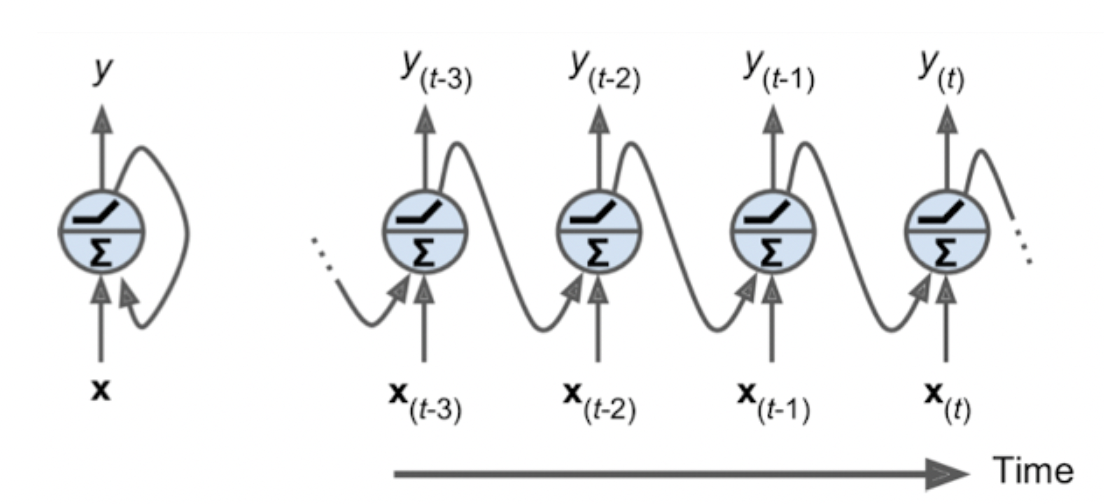
\includegraphics[width=\textwidth,height=\textheight,keepaspectratio]{Images/Theory_and_method/unnamed-6.png}
    \caption{Recurrent neurons.}
    \label{fig:Recurrent_neurons}
\end{figure}

Starting from a single RNN neuron it is possible to easily create one or more layers (Figure ~\ref{fig:RNN_multi_layer}). In more advanced models instead of using the output of a single neuron as an input for the next time step, the entire output of the layer can be used.

\begin{figure} [h]
    \centering
    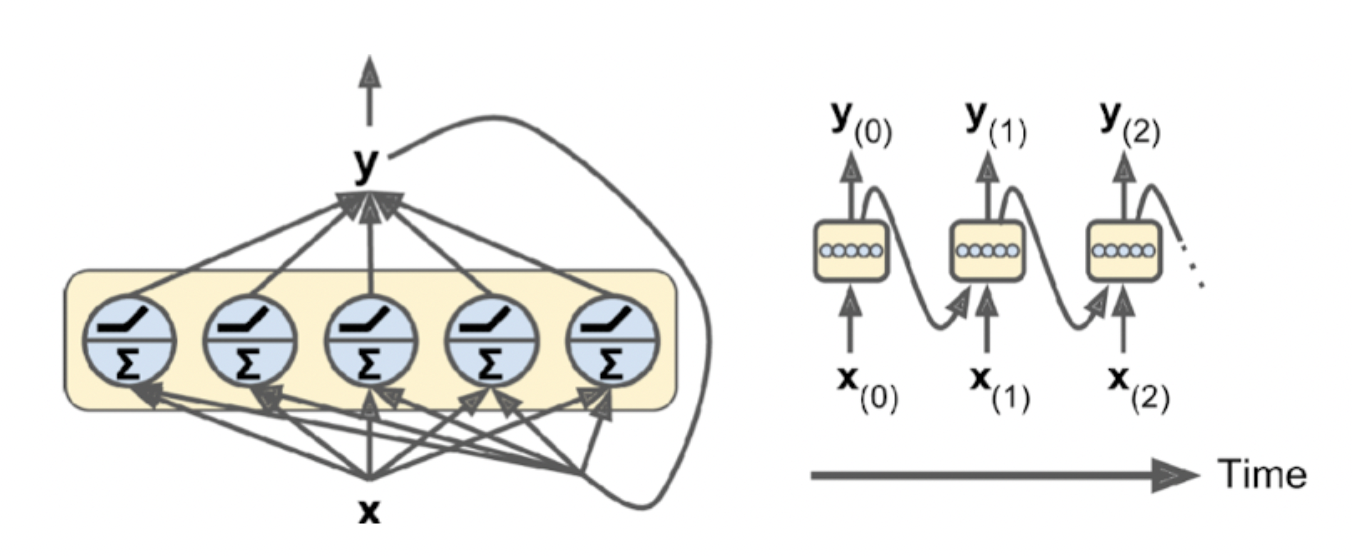
\includegraphics[width=\textwidth,height=\textheight,keepaspectratio]{Images/Theory_and_method/unnamed-7.png}
    \caption{RNN architecture with multiple neurons.}
    \label{fig:RNN_multi_layer}
\end{figure}

Each recurrent neuron has two types of weights: one for the input x(t) and the other for the output at the previous step $y_{(t-1)}$ . These two types of weights are called wx and wy, respectively. The output vector of the model is shown in Eq. \eqref{longformula}:

\begin{equation} 
   {\bf y }(t) = {\bf \phi}({\bf W}_{x}^{T} x (t) +{\bf W} _{y} ^{T} {\bf y} _{(t-1)} + {\bf b}) 
    \label{longformula}
\end{equation}

where ${\bf W}_x^T$  s the transposed version of matrix ${\bf W}_x$.

Jus like with feedforward neural network, it is possible to compute a single-step output of any given layer for  an entire batch of values by putting them all in the input matrix $X_{(t)}$ via the Eq. \eqref{longlongformula}:

\begin{equation} 
   {\bf Y} _{(t)} = {\bf \phi}({\bf X}_{(t)} {\bf W} _x + {\bf Y} _{(t-1)}{\bf W}_y + {\bf b}) = {\bf \phi}([{\bf X }_{(t)} , {\bf Y}_{(t-1)} ] {\bf W}  + {\bf b}) \: with \: {\bf W} = [{\bf W}_x ,{\bf W}_y ]^T
    \label{longlongformula}
\end{equation}

In this equation: 

\begin{itemize}
    \item ${\bf Y}_{(t)}$ is an m x $n_{neurons}$ matrix that contains the output of the layer at a given step t for each instance in the -batch (m is the number of instances, n neurons is the number of neurons).
    \item $X (t)$ is an m x n inputs matrix containing the inputs for all instances.
    \item ${\bf W}_x$ is a  $n_{inputs} \:x\: n_{neurons}$ matrix containing the connection weights for the inputs at a time t.
    \item ${\bf W}_y $ is a $n_{neurons} \:x\: n_ {neurons}$ matrix  containing the connection weights for the outputs at a previous step.
    \item ${\bf b}$ is a vector of size n, equal to the number of neurons, containing the bias of each neuron.
    Regarding the second part of the equation (compact notation):
     \item ${\bf W}$ is the vertical concatenation of the matrices ${\bf W}_x$ and ${\bf W}_y$.
    \item $[{\bf X}_{(t)}, {\bf Y}_{(t-1)}]$ represents the vertical concatenation of the matrices ${\bf X}_{(t)}$ and ${\bf Y}_{(t-1)}$.
\end{itemize}

\section{Memory Cells and long short memory term network}

\subsection{Introduction to LSTM and limits of RNN}
When using an RNN, some information is lost  or forgotten at each step. After a certain number of iterations the state of the RNN no longer contains any trace of information from the first inputs. In fact, the neurons' memory typically does not go beyond 10 steps.

It is, however, possible to extend the model in order to add memory beyond 10 steps, which is useful for doing time series forecasting, of both univariate and multivariate in nature.

\subsection{LSTM cell} \label{lstmcell}
The Long Short-Term Memory (LSTM) cell was introduced in 1997 in \citeauthor{LSTM} \autocite{LSTM}.
It offers improved performance and results compared to a other types of cells, such as RNN cells. In fact, LSTM neural networks have shorter convergence times and are also able to keep track of medium to long term dependencies in time series data such as trend and seasonality.

\begin{figure} [h]
    \centering
    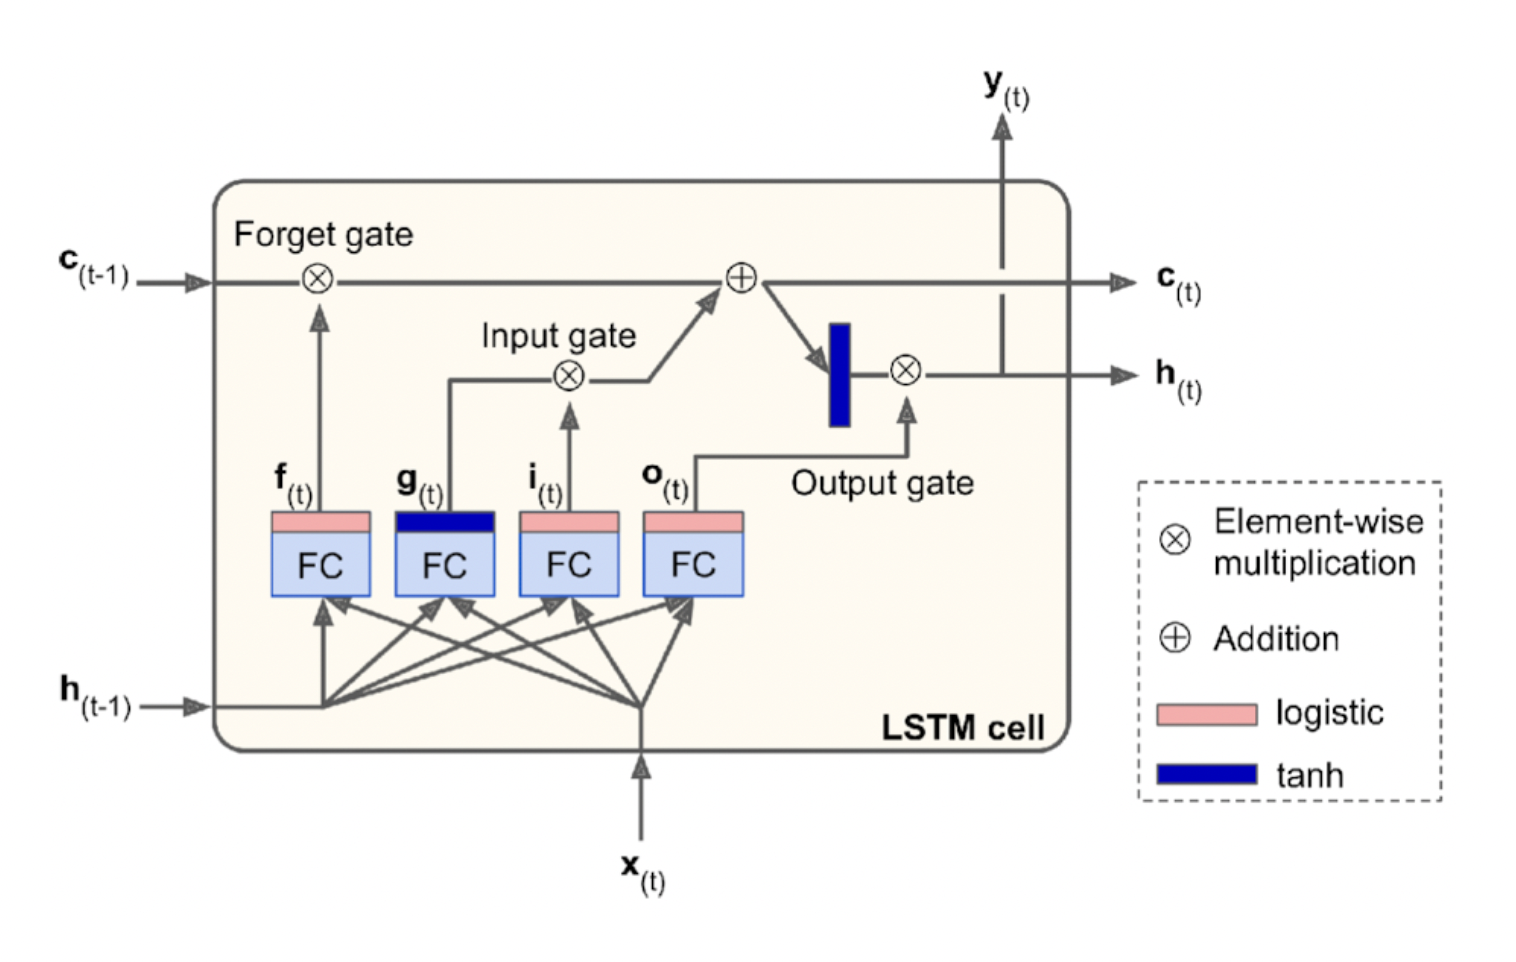
\includegraphics[width=\textwidth,height=\textheight,keepaspectratio]{Images/Theory_and_method/unnamed-8.png}
    \caption{LSTM cell.}
    \label{fig:LSTM_cell}
\end{figure}

As can be see in figure ~\ref{fig:LSTM_cell}, the cell works exactly like a classic cell, except that the state is split into 2 vectors: ${\bf h}_{(t)}$ and ${\bf c}_{(t)}$, which represent respectively the short term state and the long term state.
\begin{itemize}
    \item The main component is the one that deals with the output ${\bf g}_{(t)}$. Its activation function is a hyperbolic tangent. It deals with analyzing the input ${\bf g} {(t)}$ and the previous state ${\bf h}_{(t-1)}$. In a basic cell this would be the only component and its output would go directly to ${\bf y }_{(t)}$ and ${\bf h} _{(t)}$. In contrast, in LSTM cells the output of this cell is processed such that the most important information in the long-term state is kept and the rest of the data that is not useful is dropped. 
    \item
        The other three components are called gate controllers, because they use the logistic function as the activation function and thus their output range is between 0 and 1. Their roles are as follows: 
        \begin{itemize}
            \item ${\bf f}_{(t)}$ is called the forget gate, which defines which part of the long-term memory is to be erased. 
            \item ${\bf i}_{(t)}$ is the input gate, which determines which part of g (t) should be added to the long-term memory.
            \item ${\bf o}_{(t)}$ is called the output gate and controls which part of long-term memory should be read and added to the output, both for ${\bf h}_{(t)}$ and ${\bf y}_{(t)}$.
        \end{itemize}
\end{itemize}


Therefore, an LSTM cell can learn to recognize particularly important inputs, add them the long-term state, and store them internally until it is needed. This explains why this model has been more successful in capturing long-term patterns when it comes to time series.

 Eq. \eqref{systemformula} contains the mathematical construction of an LSTM cell.

\begin{equation} 
    \begin{array}{l}
    \mathbf{i}_{(t)}=\sigma\left(\mathbf{W}_{x i}^{\top} \mathbf{x}_{(t)}+\mathbf{W}_{h i}^{\top} \mathbf{h}_{(t-1)}+\mathbf{b}_{i}\right) \\
    \mathbf{f}_{(t)}=\sigma\left(\mathbf{W}_{x f}^{\top} \mathbf{x}_{(t)}+\mathbf{W}_{h f}^{\top} \mathbf{h}_{(t-1)}+\mathbf{b}_{f}\right) \\
    \mathbf{o}_{(t)}=\sigma\left(\mathbf{W}_{x o}^{\top} \mathbf{x}_{(t)}+\mathbf{W}_{h o}^{\top} \mathbf{h}_{(t-1)}+\mathbf{b}_{o}\right) \\
    \mathbf{g}_{(t)}=\tanh \left(\mathbf{W}_{x g}^{\top} \mathbf{x}_{(t)}+\mathbf{W}_{h g}^{\top} \mathbf{h}_{(t-1)}+\mathbf{b}_{g}\right) \\
    \mathbf{c}_{(t)}=\mathbf{f}_{(t)} \otimes \mathbf{c}_{(t-1)}+\mathbf{i}_{(t)} \otimes \mathbf{g}_{(t)} \\
    \mathbf{y}_{(t)}=\mathbf{h}_{(t)}=\mathbf{o}_{(t)} \otimes \tanh \left(\mathbf{c}_{(t)}\right)
    \end{array}
    \label{systemformula}
\end{equation}
The meanings of the terms in the equations are as follows:

\begin{itemize}
    \item  ${\bf W}_{xi} , {\bf W}_{xf} , {\bf W}_{x0}$ and $\: {\bf W}_{xg}$ are the matrices that contain the weights for each of the four components with respect to their connection to the input vector ${\bf x}_{(t)}$.
   
    \item ${\bf W}_{hi} , {\bf W}_{hf} , {\bf W}_{h0}$ and ${\bf W}_{hg}$ are the matrices that contain the weights for each of the four components with respect to their connection to the short term memory state ${\bf h}_{(t-1)}$.
    
    \item ${\bf b}_{i} , {\bf b}_{f}, {\bf b}_{0},$  and ${\bf b}_{g}$ are the bias values for each of the four components. 

\end{itemize}

\clearpage

\subsection{Other cells: Dense cells and GRU cells}
The Gated Recurrent Unit (GRU) cells were first proposed in 2014 by \citeauthor{DBLP:journals/corr/ChoMGBSB14} \autocite{DBLP:journals/corr/ChoMGBSB14}. GRU cells are a simplified version of LSTM cells, which seem to work more efficiently. The major simplifications are as follows:

\begin{itemize}
    \item The state vectors (long and short term) are combined into a single vector ${\bf h}_{(t)}$.
    \item A single gate controller ${\bf z}_{(t)}$ controls both the forgotten gate and the input gate.
    \item There is no output gate. Instead, the entire state vector is used as the output.
\end{itemize}
The schematic of the GRU cell is available in figure. ~\ref{fig:GRU_cell}:
\begin{figure} [h]
    \centering
    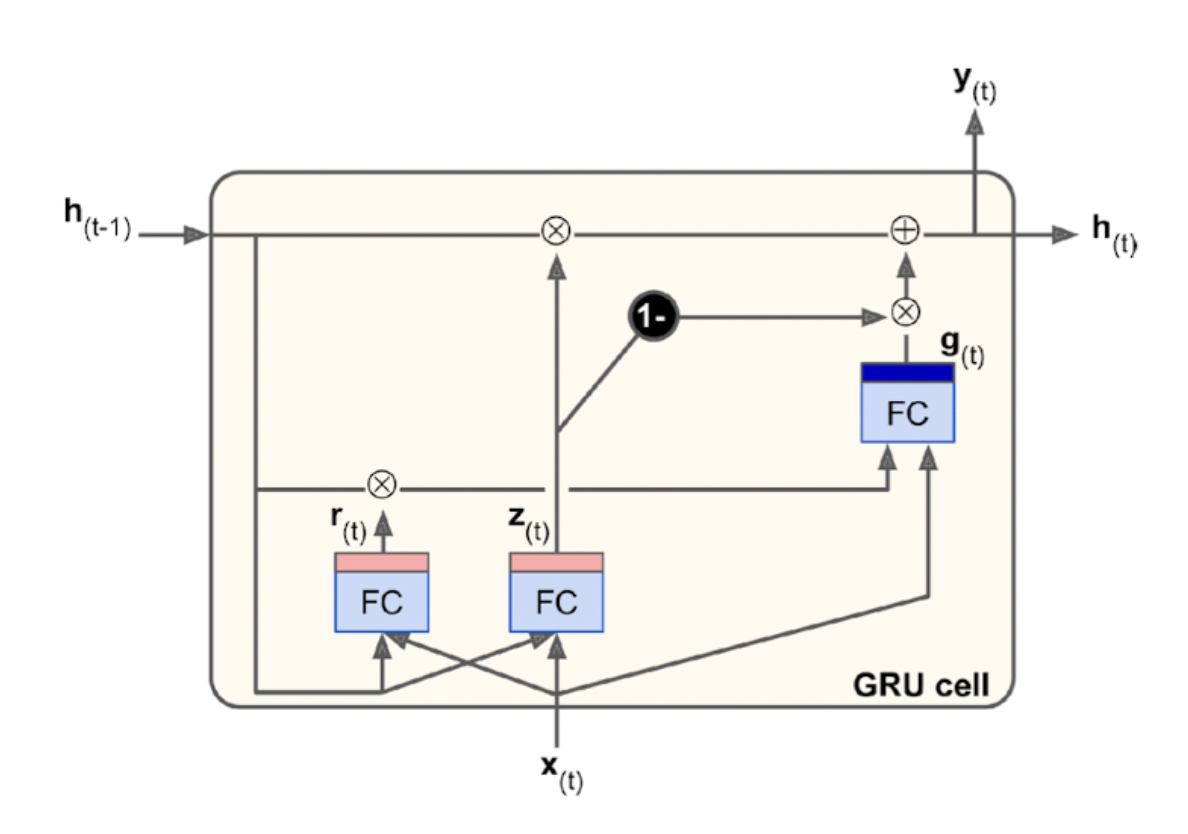
\includegraphics[width=\textwidth,height=\textheight,keepaspectratio]{Images/Theory_and_method/unnamed-9.png}
    \caption{GRU cell.}
    \label{fig:GRU_cell}
\end{figure}

\clearpage

\section{Dealing with missing values in LSTM neural networks} \label{dealwithmiss}
Traditional recurrent neural networks, including LSTM and GRU models, do not offer any inherent mechanisms to handle and learn from missing data points in any special way. On the other hand, there have been many efforts in the research field to create specialized architectures that aim to consider, and not ignore, missing values and, in doing so these efforts also tend to improve on the quality of the predictions. 

\subsection{Main strategies to address the presence of missing values}
As outlined in \citeauthor{Chollet2017-vd} \autocite{Chollet2017-vd}, there are three main techniques that can be used to extend the baseline capabilities of RNNs in the presence of missing values.

\subsubsection{Using null values}
The first and simplest approach consists of simply replacing these missing values with zeros, but this is only applicable if zero itself is not a meaningful value for the dataset. Needless to say, in the case of air quality and weather phenomena null values hold a different meaning, in that they represent instances in which data was successfully captured but either the substance is determined to be absent or the value of the weather phenomenon is zero in the given scale that it is measured with. 

That being said, in cases in which zero is indeed not a relevant value, it is expected that the network will be capable of identifying the role of this special value and therefore it is also expected that it will learn to ignore them whenever identified in out-of-sample data.
\subsubsection{Taking advantage of normalization bounds}
Given that it is often necessary to normalize or scale the data in order to speed up convergence and get values that are less prone to cause exploding gradients, whenever zero is out of the question, missing values can instead be replaced by another value, often an integer with a small absolute value, can be chosen as long as it lies outside the bounds of the scaling that has been applied to the data. 

The expected effect is the same as before: through the learning process, the special value is to be interpreted as a datapoint that must be ignored when forecasting. The fact that there is no overlap between it and the scaled data should increase the feasibility of this approach, increasing the chances that the network will learn the role of the value.

\subsubsection{Masking} \label{mask}
The third and most sophisticated solution consists of using masking. This consists of filling missing values with a predefined value often referred to as mask, just like before, this value benefits from being outside of the range of values of the dataset, and is meant to be seen by the model as a representation of a data point to ignore. The main difference in this case, however, is that the model is explicitly notified of the existence of this mask value and knows that they represent missing values from the outset, consequently circumventing the need to actually learn the role of the special value.

This can be easily integrated into previous models, in fact, the Keras implementation of TensorFlow can be extended to support the use of mask values in different types of supported types layers, like the LSTM and Dense layers that are of interest for the case study.

\section{Exploration of the hyperparameter space} \label{hyperspace}
Neural networks are often likened to black boxes, in that, especially due to the presence of hidden layers, their outputs tend not to be explainable. 
Their seemingly fickle behavior also extends to the modeling and tuning phase: while the choice of the type of neurons or cells to use can often be based on what these were originally built to do, the more specific choice of the so called hyperparameters –batch size, learning rate, number of layers, number of neurons per layers and the like– is commonly made by mere trial and error.

Different combinations of these values, using the same type of cells and the same dataset, can perform in significantly different ways, which makes testing different hyperparameters a worthwhile endeavor. Due to its nature, this phase is often referred to as the exploration of the hyperparameter space or, more concisely, hyperparameter optimization or tuning. 

This optimization process can take place following a series of different strategies that may be more or less appropriate depending on the data that they are presented with. 
\subsubsection{Grid search}
The most traditional one is called Grid Search \autocite{gridsearch} which employs an exhaustive search approach of values that come from a previously specified subset. The use of criteria to guide which types of values may yield better results is notably absent, which means that the algorithm trains all possible combinations blindly, so to speak. However, that does not immediately mean that there are no opportunities to speed up the searching process: this this process is actually what is commonly referred to as embarrassingly or delightfully parallel: the effort needed to parallelize the computational load is practically negligible, because the choice of which hyperparameters to use is independent from training processes that came before and that will come after it. 

\subsubsection{Random Search} \label{randoms}
Even better results can be obtained when applying the Random Search algorithm \autocite{JMLR:v13:bergstra12a}. This one, in fact, tackles one of the limitations of Grid Search by, as the name suggests, testing a random subset of the possible combinations, instead of systematically training all possible models in spite of their performance.

That means that in situations in which only some among all the possible hyperparameters have a significant impact on the results, this approach tends to yield better results within the same timeframe.

Random search, however, falls short from taking into account an actual choosing criterion for the hyperparameters themselves. Along with Grid Search, these algorithms select the next combination to try either by, in the case of the latter, following a previously specified order, or, in the case of the former, arbitrarily. 

\subsubsection{Optimization based approaches}
This issue is addressed by a myriad of other algorithms that use specific strategies to choose the next combination to test based on the performance of the previous ones. Said strategies can be based on the same principles that underlie the forecasting mechanisms of statistical and machine learning models. Therefore, optimization techniques, like 
\textbf{bayesian} \autocite{https://doi.org/10.48550/arxiv.1206.2944}, \textbf{gradient-based} \autocite{https://doi.org/10.48550/arxiv.1502.03492} and \textbf{evolutionary optimization} \autocite{DBLP:journals/corr/MiikkulainenLMR17} are often used for this purpose.

In all such cases, the algorithm is not forced to test combinations upon combinations of hyperparameters that yield mediocre and even worsening results. Instead, substantial amounts of time can be saved by considering values that have the potential to improve on previous results. 
Just like with any approach, however, these ones are not without their limitations: there is always the possibility of converging to local optima and, while these often present very performant results, it means that these algorithms cannot conclusively find a set of values that is guaranteed to be the best among all.

\subsubsection{Population based training}
It is important to note that parameter optimization is also the core concept that powers the predictive prowess of deep learning models, hence, there have also been efforts to combine the parameters optimization of neural networks, which is tasked with finding appropriate weights and biases, and the optimization of the hyperparameters that define that very process.

\textbf{Population based training} \autocite{DBLP:journals/corr/abs-1902-01894} extends the evolutionary approach of evolutionary optimization to train both the hyperparameters and cell weights and biases in a process that, iteratively, tries new alternatives and discards the ones that cannot match better performing fitness functions (which are any given metric used to evaluate improvements). All of this while not having to make any a-priori assumptions.

\subsubsection{Early-stopping based approaches}
The introduction of different optimization algorithms for hyperparameter tend to yield more performant results in the same amount of time, giving credence to the broader claim that using criteria to choose the next combination of hyperparameters to test is a more efficient strategy than simply going through all the different models either sequentially or at random.
However, there are different predictive mechanisms that do not solely consist of finding local optima. 

\textbf{Early stopping algorithms}, for instance, use a combination of statistical tests and random searches to determine what to evaluate next and, additionally, they owe their name to the fact that models that present early signs of low performance can be pruned, that is, removed from the pool of promising models. In doing so they spare computation time that would have been otherwise wasted, and can potentially allocate it to combinations that, according to the criteria of choice, seem more promising. 
Some implementations of this approach are \textbf{Successive Halving (SHA)} \autocite{DBLP:journals/corr/JamiesonT15} and \textbf{Asynchronous Successive Halving (ASHA)} \autocite{DBLP:journals/corr/abs-1810-05934} that prune based on statistical test results and based on performance metrics respectively. 
One more recent approach (2016), dubbed \textbf{Hyperband} \autocite{DBLP:journals/corr/LiJDRT16}, combines the previous two approaches, which allows it to cater to a wider array of applications.

\section{Deep Learning Explainability}
As far as mathematical devices go, neural networks are neither straightforward nor exceedingly complex. The core concept that powers them is matrix and vector multiplication, which is a type of operation that has been thoroughly studied and is commonly used in most other fields that use math. In fact, while certain cells, like LSTM and GRU, introduce an additional level of complexity, even these types of widely used models do not need to resort to the bleeding edge of unexplored mathematics.

And yet, despite using fundamental, well-understood notions, their application both to research and commercial applications often relies heavily on heuristic rules and trial and error in order to both train the models and interpret their results.

This leads to a seemingly paradoxical double nature: while the weights and biases of input, output and even hidden layers are readily available for inspection, they offer little to no insight as to why the model may have converged to a specific state, what modifications could lead to better results, or what are the logical steps that make a neural network arrive to a certain conclusion.

While in certain, simpler cases it may be possible to identify which parts of the input data lead to a specific output, the effect of co-dependencies among the features, the non-linearity of the model and the stochastic nature the training process tend to inhibit a clear understanding of said connections in terms of human logic. 

Statistical and other machine learning models outside the deep learning realm can clearly present information –in terms of coefficients, importance metrics, statistical significance and the like– that can potentially shine a light on the real-life motivations that tie the target phenomenon with its predictive features. Crucially, this information is often derived directly from the inner workings of the model, as is the case with regression coefficients in linear regression or splitting rules in decision trees or random forests, to name a few.

\subsection{Surrogate models}
If, on the other hand, one is to expect a certain degree of explainability coming from a neural network, more creative solutions need to be applied, that mostly rely on other models that, unlike neural networks themselves, are intrinsically explainable. 

The quintessential example of an intrinsically explainable model is simple linear regression. In this case, the beta coefficients, that act as weights in a linear combination, can be used as a metric that reflects the importance of a given feature, especially if said coefficient is deemed to be statistically significant.

In such a model, these coefficients remain the same for any given input. Thus, the resulting feature importance results are valid for the entire model, in this case the model is said to have \textbf{global fidelity} \autocite{DBLP:journals/corr/RibeiroSG16} More complex models, on the other hand, do not necessarily use the same fixed weights for every prediction: neural networks have a series of connections that can trigger, or not trigger, under different circumstances. These circumstances are shaped by the parameter tuning that takes place during the training process and make the prospect of generating a feature importance list with global fidelity an unlikely one. 

For this reason, many explainability strategies for black-box style models aim to provide instead so-called \textbf{local fidelity}, in which the validity of a feature importance value is exclusively associated to an individual prediction or output. 

One way to achieve this is by using a simpler, usually linear model as a local surrogate for the black-box model. In fact, by assuming that the behavior of the black-box model can be accurately modeled with a linear function in the vicinity of a specific data point, the resulting coefficients can be taken as a humanly comprehensible explanation as to why the overarching model produced the output in question. Moreover, by not making any further assumptions other than the feasibility of using a local linear model as a surrogate, these strategies can be described as \textbf{model agnostic}.

Two specific implementations of explainability libraries, \textbf{LIME} \autocite{DBLP:journals/corr/RibeiroSG16} and \textbf{SHAP} \autocite{DBLP:journals/corr/LundbergL17}, make use of this approach to provide a better degree of interpretability. 

\subsubsection{Lime} \label{limee}
Lime is a software library that is available for different languages like R and Python. Its name is an acronym that stands for local interpretable model-agnostic explanations and it was proposed in \citeauthor{DBLP:journals/corr/RibeiroSG16} \autocite{DBLP:journals/corr/RibeiroSG16}.

As the name implies, it aims to provide interpretability to a model’s prediction, by using localized data and by not making a priori assumptions on the nature of the model itself, ergo model-agnostic. 

Much like in the case of SHAP , the first step in achieving these claims is creating a local dataset around the chosen data point which is built from sampling values that surround it the global dataset. 

This local dataset, however, isn’t built starting directly from the original data, instead a so-called interpretable data representation is created in a series of different ways that depend on the type of data. Text, images and tabular information is supported. 

In all cases, this representation is designed to be a version of the original data that is more easily comprehensible both by experts, but especially non-experts in the field. In the case of tabular data, this is achieved by generating a weighted combination of the columns, whereas in the case of text or images, the presence or absence of words or superpixels respectively is used instead.

Having done this, the actual training set for the linear, surrogate model is created by uniformly and randomly sampling the interpretable representation and, armed with this data, the library tests the newly derived values so that it can gauge the consequent changes in the prediction. Altered features that fail to modify the result are attributed lower importance metrics compared to the ones that succeed. 

When it comes to presenting the actual importance metrics, the algorithm has to strike a balance between how well the linear model emulates the behavior of the original model, and how easily interpretable the information can be. 

\begin{equation} 
  \xi(x)=\underset{g \in G}{\operatorname{argmin}} \mathcal{L}\left(f, g, \pi_{x}\right)+\Omega(g)
    \label{davidEquation}
\end{equation}

This is achieved by minimizing \eqref{davidEquation}, which is composed of the sum of two terms. 

The first one, called \textbf{locality-aware loss}, gives an indication as to how well the linear model adapts to the black-box one. It depends on the explanatory model g, a proximity measure π that indicates the distance between the data point in question, x, and the perturbed values that are used to train the explanatory model, and the original predictor model f. 

The second one, called \textbf{measure of model complexity}, indicates how complex the ensuing interpretations are from a human perspective. It therefore depends on the type of intrinsically explainable model of choice: for linear regression it could be the amount of statistically significant coefficients.

Minimizing the first term, therefore, increases local fidelity; minimizing the second one increases the perceived explainability of the model. 

\subsubsection{SHAP}
\textbf{SHAP} is another software library that provides functionality similar to LIME’s. It is model-agnostic and provides explanations with local fidelity. 
The novelty that SHAP brings to the table is the use of Shapley values, a game-theory concept that is the key to replacing the use of surrogate linear models, eliminating the possibility of having to compromise local fidelity in exchange for explainability. 

Shapley values were originally proposed by mathematician and economist Lloyd Shapley \autocite{RM-670-PR}–who later went on to win the Nobel prize For Economic Sciences in 2012 due to this very same contribution– as an indicator that can be calculated to determine the contribution of each player in a game, especially when these work together in coalitions. 

In other words, a metric for the marginal contribution of each player is calculated by perturbing the input of each player and comparing the result to an unperturbed baseline. These marginal contributions are then presented as an average, which is calculated by attributing different weights to the difference between the contribution of a coalition without a given player and the contribution of the same coalition with said player as a part of it.

The fraction represents the weight of the respective marginal contribution, whereas the first term in the subtraction represents the contribution of the coalition with the player in it, and the second term the same contribution without it. 

\begin{equation} 
    \Phi_{i}(v)=\sum_{S \subseteq N \backslash\{i\}} \frac{|S| !(N-|S|-1) !}{N !}(v(S \cup\{i\})-v(S))
    \label{LongdavidEquation}
\end{equation}

When applied to machine learning, the players become the features or predictors, and the average marginal contribution measured by the Shapley values is associated with the output of the model, and how each one of these features contributes to it. Coalitions are therefore combinations of features with respect to which the contribution of a given predictor is measured. 
The implementation of said coalitions for machine learning models represents both an interesting opportunity for explainability, but also one of the biggest disadvantages of Shapley values. 

Indeed, this strategy allows for the evaluation of every single predictor against its impact in the context of different groups of other predictors, which shines a line on how its contribution can change as a function of its interaction with other features. 

Yet, the amount of subsets of features that need to be taken into account increases exponentially with each additional feature, making the computational cost of Shapley values all too high when no approximations are used.

In addition to the need for approximation to deal with high amounts of features, the use of Shapley values for machine learning requires one additional modification. While the theoretical definition of their calculation requires the exclusion of the feature that is being tested for the baseline prediction, it is not possible to simply exclude it when calculating the predictions with neural networks or random forests and the like. The solution used in practice consists of sampling the distribution of the feature itself and then averaging its value across different samples. This can be done in different ways that are more or less computationally expensive and that differentiate all the different libraries that use Shapley values. 

\subsubsection{Local fidelity and global explainability}

Both Lime and SHAP produce explanations that can be tied to the actual behavior of the black-box model only in the vicinity of the chosen data point. In fact, either by creating a local linear model or by calculating the Shapley values for a certain input, the indicators that are produced only consider the behavior of the original model for the chosen data point, and not its global behavior.

It may be, therefore, tempting to calculate these local explanations for multiple data points, so that all-encompassing conclusions can be drawn from them. 

If a subset of inputs is chosen so that the data is representative of the entire domain of input values, the features that come up as having high importance more often than not may be considered to be more relevant to the predictions. 

While identifying features that are consistently crucial is, without a doubt, useful to form a better understanding of the model’s choices, this must not be confused with the concept of global fidelity. 

An explanation that attains global fidelity is one that accurately explains the choices of the model in all circumstances, whereas the above proposal only constitutes a qualitative assessment, and cannot guarantee that a predictor will be more or less relevant than the others in all cases, unless all possible inputs are tested and this is shown to be the case. The domain of possible inputs, however, is, more often than not, infinite, hence true global fidelity is not feasible with these approaches.

\chapter{Other models} \label{othermod}
\section{Random forest} \label{randomfor}
Random forests are a famous type of machine learning model created by \citeauthor{Breiman2001} \autocite{Breiman2001} that involves combining the output of multiple decision trees to obtain a single result. It is used for both classification and regression problems.

It is based on collections of decision trees (hence the name forest) that are split recursively in a binary fashion until the leaf is reached by simple comparison. 

Each decision tree is constructed by taking data randomly from the source dataset; this step is called bootstrapping.
\section{Multiple linear regression with ARIMA errors}
One of the most commonly used models used for time-series forecasting are the multiple regression models with ARIMA errors \autocite{TimeSeries}. Being statistical as a benchmark to compare the performance of these two different types of models.   